\onecolumn
\chapter{Auswertung}
% Liste der genutzer Formeln für die Fehlerrechnung
\section*{Fehlerrechnung}
Für die statistische Auswertung von $n$ Messwerten $x_i$ werden folgende Größen definiert \cite{errorSkript25}:
\begin{align}
    \bar{x} &= \frac{1}{n} \sum_{i=1}^{n} x_i \vphantom{\sqrt{\sum_i^n}^2} && \text{\textcolor{gray}{Arithmetisches Mittel}} \label{eq:arithmetisches_mittel} \\
    \sigma^2 &= \frac{1}{n-1} \sum_{i=1}^{n} (x_i - \bar{x})^2 \vphantom{\sqrt{\sum_i^n}^2} && \text{\textcolor{gray}{Variation}} \label{eq:variation} \\
    \sigma &= \sqrt{\frac{1}{n-1} \sum_{i=1}^{n} (x_i - \bar{x})^2} \vphantom{\sqrt{\sum_i^n}^2} && \text{\textcolor{gray}{Standardabweichung}} \label{eq:standardabweichung} \\
    \Delta \bar{x} &= \frac{\sigma}{\sqrt{n}} = \sqrt{\frac{1}{n(n-1)} \sum_{i=1}^n(\bar x - x_i)^2} \vphantom{\sqrt{\sum_i^n}^2} && \text{\textcolor{gray}{Fehler des Mittelwerts}} \label{eq:fehler_mittelwert} \\
    \Delta f &= \sqrt{\left(\frac{\partial f}{\partial x} \Delta x\right)^2 + \left(\frac{\partial f}{\partial y} \Delta y\right)^2} \vphantom{\sqrt{\sum_i^n}^2} && \text{\textcolor{gray}{Gauß’sches Fehlerfortpflanzungsgesetz für $f(x,y)$}} \label{eq:gauss_fehlfortpflanzung} \\
    \Delta f &= \sqrt{(\Delta x)^2 + (\Delta y)^2} \vphantom{\sqrt{\sum_i^n}^2} && \text{\textcolor{gray}{Fehler für $f = x + y$}} \label{eq:fehler_summe} \\
    \Delta f &= |a| \Delta x \vphantom{\sqrt{\sum_i^n}^2} && \text{\textcolor{gray}{Fehler für $f = ax$}} \label{eq:fehler_proportional} \\
    \frac{\Delta f}{|f|} &= \sqrt{\left(\frac{\Delta x}{x}\right)^2 + \left(\frac{\Delta y}{y}\right)^2} \vphantom{\sqrt{\sum_i^n}^2} && \text{\textcolor{gray}{relativer Fehler für $f = xy$ oder $f = x/y$}} \label{eq:relativer_fehler} \\
    \sigma &= \frac{|a_{lit} - a_{gem}|}{\sqrt{\Delta a_{lit}^2 + \Delta a_{gem}^2}} \vphantom{\sqrt{\sum_i^n}^2} && \text{\textcolor{gray}{Berechnung der signifikanten Abweichung}} \label{eq:signifikante_abweichung}
\end{align}

\twocolumn

\section{Berechnung des Wasserwertes}
Wir beginnen mit der \hyperref{eq:wasserwert}{Berechnung des Wasserwertes}. 
Hierfür benötigen wir zwei Referenztemperaturen. Wir nutzen einmal die Zimmertemperatur $T_2 =25,1 ^\circ C$. Wir sind dabei von einer Unenaugigkeit des Thermometers von $^1\circ C$ ausgegangen.
Wichtig für die Rechnung werden wie Werte aus \hyperref[Prtokoll]{Tabelle 2 des Prtokolls}. Hier sind zwei Messreihen aufgeführt.
Dabei wurde die zweite Messreihe durchgeführt, da wir bei der ersten die Durchführung nicht genau genug beachtet hatten. Die grauen Werte sind dabei immer die der ersten Messreihe.
In der Gleichung des Wasserwertes kommt die spezifische Wärmekapazität des Wassers drinnen vor, dafür nutzen wir den Literaturwert von
$c_w = (4,186 \pm 0,004) \frac{J}{g \cdot k}$. Zur bestimmung der Masse des Wassers $m_w$ wurde das Kalorimeter ohne Deckel einmal leer $m_l$ und mit Wasser gefüllt $m_v$ gewogen.
Zieht man die differenz beider, so kommt man auf eine Masse von:
\begin{equation}
    m_w = 354,2 g.
\end{equation}

Diesen Wert können wir aber nicht einfach so übernehmen, wir müssen noch seine Ungenauigkeit bestimmen. Die Messungenauigkeit der Waage liegt dabei bei $\Delta m = 0,1g$. Dieser Fehler gilt für beide Massen.
Über die \hyperref[eq:gauss_fehlfortpflanzung]{Gauß'che Fehlerfortpflanzung} kommt man somit eine Ungenauigkeit
\begin{equation}
    \Delta m_w = \sqrt{\Delta {m_l} ^2 + \Delta {m_v} ^2} = 0,141g.
\end{equation}

Fügen wir das zusammen, haben wir eine Wassermasse von
\begin{equation}
    m_w = (354,2 \pm 0,14)g.
\end{equation}

Wir haben bei der zweiten Messreihe extra darauf geachtet, die möglichst exakt gleich Masse zu erreichen. 
Für den Wasserwert brauchen wir aber noch einen zweiten Referenzwert, $T_1$.
Das Thermometer weist einen Fehler von \(\pm(0{,}3\,\% + 1\,\si{\celsius})\) auf. Systematische Fehler, die absolute Temperaturmessungen verzerren, sind hierin vermutlich bereits berücksichtigt. Da in diesem Versuch nur Temperaturdifferenzen relevant sind, auf die systematische Abweichungen kaum Einfluss haben, wird hier ausschließlich der relative Fehler von \(0{,}3\,\%\) des Messwerts angesetzt.
Der Wert $T_1$ ist dem \hyperref[Prtokoll]{Protokoll, Tabelle 2} zu entnehmen:
\begin{align}
    T_1 = (50,0 \pm 0,15)^\circ C \\ 
    \notag \textcolor{gray}{T_1 = (50,5 \pm 0,15)^\circ C}.
\end{align}

Der \hyperref[fig:temp_against_time]{Abbildung 3.1} sind die Werte
\begin{align}
    \overline{T_A} = 49,09^\circ C  \text{ und}\\
    \overline{T_F} = 49,18^\circ C
\end{align}
zu entnehmen. Dabei berechnet sich die Ungenauigkeit zu
\begin{equation}
    \Delta \bar{T} = \left| \overline{T_A} - \overline{T_F} \right| = 0,09 [^\circ C].
\end{equation}

Zusammengefügt wird dies zu:
\begin{equation}
    \bar{T} = (49,09 \pm 0,09) ^\circ C.
\end{equation}

Mit diesen Werten können wir schonmal den Wasserwert berechnen:
\begin{equation}
    W = 354,2 \cdot 4,186 \frac{0,91}{23,99} = 56,24176 \frac{J}{K}
\end{equation}

Müssen wir noch die Ungenauigkeit bestimmen. Wir nutzen wieder die \hyperref[eq:gauss_fehlfortpflanzung]{Gauß'che Fehlerfortpflanzung}:
\begin{equation}
    \Delta W = 
    \sqrt{
    \begin{aligned}
    &\left( c_W \frac{T_1 - \overline{T}}{\overline{T} - T_2} \Delta m_W \right)^2 \\
    &+ \left( m_W \frac{T_1 - \overline{T}}{\overline{T} - T_2} \Delta c_W \right)^2 \\
    &+ \left( m_W c_W \frac{1}{\overline{T} - T_2} \Delta T_1 \right)^2 \\
    &+ \left( - m_W c_W \frac{T_1 - \overline{T}}{(\overline{T} - T_2)^2} \Delta T_2 \right)^2 \\
    &+ \left( m_W c_W \frac{T_2 - T_1}{(\overline{T} - T_2)^2} \Delta \overline{T} \right)^2
    \end{aligned}
    }
    \label{eq:deltaW}
\end{equation}

Setzen wir alles in diese Formel ein, so kommen wir auf
\begin{equation}
    \Delta W = 11,1714 \frac{J}{K}.
\end{equation}

Noch zu einem Ergebnis zusammenfügen:
\begin{equation}
    \boxed{W = (56,24 \pm 11,17) \frac{J}{K}}
\end{equation}
\begin{equation*}
    \textcolor{gray}{
        \boxed{W = (9 \pm 54) \frac{J}{K}}
    }
\end{equation*}

\onecolumn
\begin{figure}
    \centering
    \includegraphics[width=\textwidth, page=4]{Protokolle/\versuchsnummer/Chapter/Messprotokoll.pdf}
    \caption{Resonance curve for weak dumping (340mA). The red line is the maximum $\omega'$ and orange is the half-width $H$.}
    \label{fig:temp_against_time}
\end{figure}
\twocolumn


Es ist sehr eindeutig, dass die Ertse Messreihe misslungen ist, und keinen Sinn ergibt.

\section{Berechnung spezifische Wärmekapazität im Kalorimeter}
Wir bestimmen nun die spezifische Wärme der drei Probematerialien (Aluminium (Al), Blei (Pb) und Graphit (C-Verbindung)). 
Doch zunächst müssen wir bestimmen, wie warm das kochende Wasser tatsächlich war; denn die $100^\circ C$ gelten bei einem Normaldruck $p_0 = 1013 hPa$.
Daher rechnen wir unsere tatsächliche Temperatur aus:
\begin{equation}
    T_1(p) = 100^\circ C + 0,0276 \frac{^\circ C}{hPa} \cdot (p-p_0).
    \label{eq:temp_corecctur}
\end{equation}

Wir haben dabei einen Luftdruck von $P = 1001,2$ hPa abgelesen, und gehen von einer Ungenauigkeit von $\Delta p = 0,5 hPa$.
Setzen wir diese Werte in die \hyperref[eq:temp_corecctur]{Gleichung} ein, so kommen wir auf:
\begin{equation}    
    T_1 = 99,674 ^\circ C.
\end{equation}

Die Ungenauigkeit berechnet sich über:
\begin{equation}
    \Delta T_1 = 0,0276 {^\circ C}{hPa} \cdot \Delta p = 0,0138,
\end{equation}

somit kommen wir auf ein Ergebnis von
\begin{equation}
    \underline{T_1 = (99,674 \pm 0,014)^\circ C}.
\end{equation}

Wir berechnen nun die \hyperref[eq:spezifische_waermekapazitaet]{spezifische Wärme}. Dafür müssen wir jedaoch auch 
die Ungenauigkeit über die \hyperref[eq:gauss_fehlfortpflanzung]{Gauß'che Fehlerfortpflanzung} bestimmen:

\begin{equation}
    \Delta c_x = 
    \sqrt{ 
    \begin{aligned}
    &   \left( \frac{c_W ( \overline{T} - T_2)}{T_1 - \overline{T}} \frac{1}{m_x} \Delta m_W \right)^2 \\
    & + \left( \frac{m_W (\overline{T} - T_2)}{T_1 - \overline{T}} \frac{1}{m_x} \Delta c_W \right)^2 \\
    & + \left( \frac{\overline{T} - T_2}{(T_1 - \overline{T}) m_x} \Delta W \right)^2 \\
    & + \left( \frac{c_x \Delta m_x}{m_x} \right)^2 \\
    & + \left( - \frac{(T_1 - T_2)(c_W m_W + W)}{m_x (T_1 - \overline{T})^2} \Delta \overline{T} \right)^2 \\
    & + \left( \frac{(c_W m_W + W)}{m_x (\overline{T} - T_2)} \Delta T_1 \right)^2 \\
    & + \left( \frac{c_x \Delta T_2}{\overline{T} - T_2} \right)^2
    \end{aligned}
    }
    \label{eq:deltacx}
\end{equation}

Wir nutzen für $\Delta T_1$ die Angaben des Thermometerherstellers: $\Delta T_1 = \pm(0,3\% + 1^\circ C)$.
Wir stellen die Ergebnisse \hyperref[tab:waermekapazitaeten]{Tabellarisch} dar:
\onecolumn
\begin{table}[h!]
    \centering
    \begin{tabular}{l | l | l | l}
        \toprule
        Größe & Graphit & Blei & Aluminium \\
        \hline
        $T_2 [^\circ C]$ & $33,5 \pm 1$ & $30,8 \pm 1$ & $25,5 \pm 1$ \\
        $\overline{T} [^\circ C]$ & $36,6 \pm 0,09$ & $33,3 \pm 0,09$ & $30,5 \pm 0,1$ \\
        $m_w [g]$ & $372,2 \pm 1$ & $373 \pm 1$ & $373,2 \pm 1$ \\
        $m_x [g]$ & $122,2 \pm 1$ & $618,3 \pm 1$ & $148,9 \pm 1$ \\
        $M [\mathrm{g/mol}]$ & $12,01$ & $207,2$ & $26,98$ \\
        \midrule
        $c_x [\mathrm{J/g \cdot K}]$ & $0,64926 \pm 0,21878$ & $0,09854 \pm 0,04222$ & $0,64926 \pm 0,16175$ \\
        $c_\mathrm{mol} [\mathrm{J/mol \cdot K}]$ & $8 \pm 3$ & $20 \pm 9$ & $19 \pm 4$ \\
        \bottomrule
    \end{tabular}
    \caption{Messwerte und Unsicherheiten für Graphit, Blei und Aluminium}
    \label{tab:waermekapazitaeten}
\end{table}
\twocolumn







\section{Berechnung spezifische Wärme (Kalt)}